%%%%%%%%%%%%%%%%%%%%%%%%%%%%%%%%%%%%%%%%%
% Beamer Presentation
% LaTeX Template
% Version 1.0 (10/11/12)
%
% This template has been downloaded from:
% http://www.LaTeXTemplates.com
%
% License:
% CC BY-NC-SA 3.0 (http://creativecommons.org/licenses/by-nc-sa/3.0/)
%
%%%%%%%%%%%%%%%%%%%%%%%%%%%%%%%%%%%%%%%%%

%------------------------------------------------------------------------------------------------
% PACKAGES AND THEMES
%------------------------------------------------------------------------------------------------

\documentclass[table, xcolor = {dvipsnames}, 9pt]{beamer}
\usepackage{tikz}
\usetikzlibrary{calc}
\usetikzlibrary{positioning}
\usetikzlibrary{arrows.meta}
\usetikzlibrary{external}
\mode<presentation> {

% The Beamer class comes with a number of default slide themes
% which change the colors and layouts of slides. Below this is a list
% of all the themes, uncomment each in turn to see what they look like.

\usetheme{default}
%\usetheme{AnnArbor}
%\usetheme{Antibes}
%\usetheme{Bergen}
%\usetheme{Berkeley}
%\usetheme{Berlin}
%\usetheme{Boadilla}
%\usetheme{CambridgeUS}
%\usetheme{Copenhagen}
%\usetheme{Darmstadt}
%\usetheme{Dresden}
%\usetheme{Frankfurt}
%\usetheme{Goettingen}
%\usetheme{Hannover}
%\usetheme{Ilmenau}
%\usetheme{JuanLesPins}
%\usetheme{Luebeck}
%\usetheme{Madrid}
\usetheme{metropolis}
%\usetheme{Malmoe}
%\usetheme{Marburg}
%\usetheme{Montpellier}
%\usetheme{PaloAlto}
%\usetheme{Pittsburgh}
%\usetheme{Rochester}
%\usetheme{Singapore}
%\usetheme{Szeged}
%\usetheme{Warsaw}

% As well as themes, the Beamer class has a number of color themes
% for any slide theme. Uncomment each of these in turn to see how it
% changes the colors of your current slide theme.

%\usecolortheme{albatross}
%\usecolortheme{beaver}
%\usecolortheme{beetle}
%\usecolortheme{crane}
%\usecolortheme{dolphin}
%\usecolortheme{dove}
%\usecolortheme{fly}
%\usecolortheme{lily}
%\usecolortheme{orchid}
%\usecolortheme{rose}
\usecolortheme{seagull}
%\usecolortheme{seahorse}
%\usecolortheme{whale}
%\usecolortheme{wolverine}
\usefonttheme{professionalfonts}
%\setbeamertemplate{footline} % To remove the footer line in all slides uncomment this line
%\setbeamertemplate{footline}[page number] % To replace the footer line in all slides with a simple slide count uncomment this line

%\setbeamertemplate{navigation symbols}{} % To remove the navigation symbols from the bottom of all slides uncomment this line
}

\usepackage{graphicx} % Allows including images
\usepackage{booktabs} % Allows the use of \toprule, \midrule and \bottomrule in tables
\usepackage{tikz}
\usepackage{multirow}
\usepackage{natbib}
\usepackage{hyperref}
\usepackage{diagbox}
\usepackage{makecell}
\usepackage{xparse}
\usepackage{subfig}
\usepackage{amsmath}
\usepackage{amsfonts,amsthm,amsmath,amssymb}    
\usepackage{bbm}
\usepackage{bm}
\usepackage{empheq}
\usepackage{pgfplots}
\usepackage{animate}
\usepgfplotslibrary{colorbrewer}

\newcommand\mybox[2][]{\tikz[overlay]\node[fill=lightgray,inner sep=2pt, anchor=text, rectangle, rounded corners=1mm,#1] {#2};\phantom{#2}}
\hypersetup{unicode=true,
            bookmarksnumbered=true,
            bookmarksopen=true,
            bookmarksopenlevel=2,
            breaklinks=false,
            pdfborder={0 0 1},
            hypertexnames=false,
            pdfstartview={XYZ null null 1}}
\usepackage{xcolor}
\newcommand\myheading[1]{%
  \par\bigskip
  {\Large\bfseries#1}\par\smallskip}
\newcommand\given[1][]{\:#1\vert\:}
\theoremstyle{plain}
\newtheorem{thm}{Theorem}
\newtheorem{prop}{Proposition\thisthmnumber}
\newtheorem{lem}{Lemma\thisthmnumber}
\newtheorem{cor}{Corollary}
\newtheorem{defin}{Definition}
\newtheorem{algo}{Algorithm}
\newcommand*\diff{\mathop{}\!\mathrm{d}}
\newcommand*\Diff[1]{\mathop{}\!\mathrm{d^#1}}
\newcommand{\bh}[1]{{\color{blue}{#1}}}
\newcommand{\mh}[1]{{\color{magenta}{#1}}}
\newcommand{\thisthmnumber}{}
\newcommand{\tikzmark}[1]{\tikz[baseline,remember picture] \coordinate (#1) {};}
\newcommand*{\QEDA}{\hfill\ensuremath{\blacksquare}}%
\newcommand*{\QEDB}{\hfill\ensuremath{\square}}%
\DeclareMathOperator{\E}{\rm{E}}
\DeclareMathOperator{\R}{\mathbb{R}}
\DeclareMathOperator{\N}{\mathbb{N}}
\DeclareMathOperator{\Var}{\rm{Var}}
\DeclareMathOperator{\Cov}{\rm{Cov}}
\DeclareMathOperator{\Supp}{\rm{Supp}}
\DeclareMathOperator{\e}{\rm{e}}
\DeclareMathOperator{\F}{\mathcal{F}}
\DeclareMathOperator{\Z}{\mathcal{Z}}
\DeclareMathOperator{\logit}{\rm{logit}}
\DeclareMathOperator{\indep}{{\perp\!\!\!\perp}}
\DeclareMathOperator{\rank}{rank}
\DeclareMathOperator*{\argmin}{arg\,min}
\DeclareMathOperator*{\argmax}{arg\,max}
%\DeclareMathOperator{\Pr}{\rm{Pr}}
%------------------------------------------------------------------------
% TITLE PAGE
%-----------------------------------------------------------------------
\pagestyle{empty}
\title[]{Regression Discontinuity Design} % The short title appears at the bottom of every slide, the full title is only on the title page

\author{Thomas Leavitt} % Your name
\institute[] % Your institution as it will appear on the bottom of every slide, may be shorthand to save space
{
% Your institution for the title page
\medskip
\textit{} % Your email address
}
\date{August 8, 2022} % Date, can be changed to a custom date

\begin{document}

\begin{frame}
\titlepage % Print the title page as the first slide
\end{frame}

%\begin{frame}
%\frametitle{Overview} % Table of contents slide, comment this block out to remove it
%\tableofcontents % Throughout your presentation, if you choose to use \section{} and \subsection{} commands, these will automatically be printed on this slide as an overview of your presentation
%\end{frame}

%------------------------------------------------------------------------
% PRESENTATION SLIDES
%----------------------------------------------------------------
\section{Overview}
\begin{frame}
\frametitle{Overview: Regression Discontinuity Design (RDD)} 
\begin{itemize} \vfill
\item Applicable when treatment assigned according to known
\textit{rule} or \textit{threshold} (e.g., administrative programs, elections) \vfill
\item An idea that goes back to \citet{thistlethwaitecampbell1960}: \vfill 
\begin{itemize} \vfill
\item What are effects of college scholarships on students' achievement? \vfill
\item Scholarships awarded on basis of whether test score exceeds threshold $c$ \vfill
\item Treatment $Z_i$ is scholarship \vfill
\item Running variable $X_i$ is test score score with cutoff $c$ \vfill
\item Outcome $Y_i$ is subsequent earnings \vfill
\item $Y_i(0)$: potential earning without scholarship \vfill
\item $Y_i(1)$: potential earning with scholarship \vfill
\item $Y_i(1)$ and $Y_i(0)$ are related to $X_i$: On average, students with higher test scores would obtain higher earnings \vfill
\end{itemize} \vfill
\end{itemize} \vfill
\end{frame}
%----------------------------------------------------------------
\begin{frame}
\frametitle{Overview: Regression Discontinuity Design (RDD)} 
\begin{itemize} \vfill
\item Two frameworks of RDDs: \vfill
\begin{enumerate} \vfill 
\item Local as-if random assignment \\ \citep{cattaneoetal2015,saleshansen2020} \vfill
\begin{itemize} \vfill
\item Causal target: Weak or sharp effect among units in window around cutoff \vfill
\item Key assumption: As-if random assignment in window around cutoff \vfill
\end{itemize} \vfill
\item Continuity-based framework \\ \citep{hahnetal2001,imbenslemieux2008} \vfill
\begin{itemize} \vfill
\item Causal target: Average effect at cutoff \vfill
\item Key assumption: Continuity of potential outcomes' conditional expectations \vfill
\end{itemize} \vfill
\end{enumerate} \vfill
\end{itemize} \vfill
\end{frame}
%----------------------------------------------------------------
\section{General setup}
\begin{frame}
\frametitle{Setup: Regression Discontinuity Design} 
\begin{itemize} \vfill
\item Units: $i \in \{1, \ldots, n\}$
\item $Z_i \in \{0,1\}$: Treatment
\item Potential outcomes: $Y_i(0)$ and $Y_i(1)$
\item Observed outcome: $Y_i = Z_i Y_i(1) + (1-Z_i) Y_i(0)$ 
\item $X_i$: \bh{Running variable} perfectly determines value of $Z_i$ with cutpoint $c$
\begin{equation*}
Z_i = \mathbbm{1}\{X_i \geq c\} \quad \text{or, equivalently,} \quad Z_i = \left\{
\begin{array}{ll}
1 & \mbox{if $X_i \geq c$}\\
0 & \mbox{if $X_i < c$}
\end{array}
\right.
\end{equation*} \vfill
\item $X_i$ may be correlated with $Y_i(0)$ and $Y_i(1)$ \vfill
\item Treatment is deterministic function of running variable \vfill
\end{itemize} \vfill
\end{frame}
%----------------------------------------------------------------
\begin{frame}
\frametitle{Setup: Regression Discontinuity Design} 
\vfill
\begin{center}
\includegraphics[height=.8\textheight]{figures/treatment_plot.pdf}
\end{center}
\vfill
\begin{itemize} \vfill
\item Scores $<$ cutoff $\rightarrow$ control; scores $\geq$ cutoff $\rightarrow$ treatment \vfill
\end{itemize} \vfill
\end{frame}
%----------------------------------------------------------------
\section{Local as-if random assignment}
\begin{frame}
\frametitle{Local as-if random assignment} 
\vfill
\begin{itemize} \vfill
\item \bh{Key assumption}: As-if random assignment in window around cutoff \vfill
\item[] For all $i \in \left\{1, \ldots , n\right\}$, independent and identical distributions of \vfill
\begin{align*}
\left(X_i \given W_i = 1\right), \text{ where } W_i = \mathbbm{1}\left\{c - \underline{h} \leq X_i \leq c + \overline{h}\right\}
\end{align*} \vfill
\item \mh{Note}: $\underline{h} > 0$ and $\overline{h} > 0$ are used for lower and upper bounds of window around cutoff \vfill
\item In words: The probability that running variable takes on each value in window around cutoff is same for all units \vfill
\item[] This assumption $\implies$ independent and identical distributions of $Z_1, \ldots , Z_n$ \vfill
\item Plausibility of as-if randomness assessed by comparison to distribution of covariate balance in randomized experiment \citep{hansenbowers2008} \vfill
\end{itemize} \vfill
\end{frame}
%----------------------------------------------------------------
\subsection{Exclusion restriction}
\begin{frame}
\frametitle{Exclusion restriction} 
\vfill
\begin{itemize} \vfill
\item Treatment is deterministic function of running variable \vfill
\item[] $\rightarrow$ treatment and control \textbf{cannot} be balanced on running variable \vfill
\item Running variable may be related to potential outcomes \vfill
\item[] $\rightarrow$ need to assume running variable affects POs through only treatment \citep{sekhontitiunik2017} \vfill
\item \bh{Exclusion restriction}: For all $i \in \left\{1, \ldots , n\right\}$, \vfill 
\item[] $Y_i(0)$ fixed for all $X_i \in [c - \underline{h}, c)$ and $Y_i(1)$ fixed for all $X_i \in [c, c + \overline{h}]$ \vfill
\end{itemize} \vfill
\end{frame}
%----------------------------------------------------------------
\subsection{Bandwidth selection}
\begin{frame}
\frametitle{Bandwidth selection} 
\begin{itemize} \vfill
\item ``Stepwise intersection-union principle'' (SIUP) \\ \citep{hansensales2015,rosenbaum2008,berger1988} \vfill
\item[] ``if a researcher pre-specifies a sequence of hypotheses and corresponding level-$\alpha$ tests, tests those hypotheses in order, and stops testing after the first non-rejected hypothesis, then the probability of incorrectly rejecting at least one correct hypothesis is at most $\alpha$'' \citep[p. 185]{hansensales2015}. \vfill
\item For RDDs \vfill
\begin{enumerate} \vfill
\item Start with a set of candidate bandwidths \vfill
\item Sequentially test for covariate balance (beginning from either largest or smallest candidate bandwidth) \vfill
\item Stop testing after first bandwidth with $p$-value equal or greater than pre-determined $\alpha$-level for covariate balance \vfill
\end{enumerate} \vfill
\end{itemize} \vfill
\end{frame}
%----------------------------------------------------------------
\begin{frame}
\frametitle{Bandwidth selection} 
\vfill
\begin{center}
\includegraphics[height=.8\textheight]{figures/cov_bal_bandwidth.pdf}
\end{center}
\vfill
\end{frame}
%----------------------------------------------------------------
\subsection{Estimation and inference}
\begin{frame}
\frametitle{Estimation and inference} 
\vfill
\begin{itemize} \vfill
\item Same tools for estimation and testing of weak or sharp effects from Week 1 \vfill
\item Can also include additional step of detrending control POs \\ \citep{saleshansenrowan2018,saleshansen2020} \vfill
\begin{enumerate} \vfill
\item Fit model of control POs as function of running variable to data below cutoff \vfill
\item Use fitted model to predict and detrend outcomes below and above cutoff \vfill
\item Conduct inference on residuals (detrended outcomes) \vfill
\end{enumerate} \vfill
\end{itemize} \vfill
\end{frame}
%----------------------------------------------------------------
\begin{frame}
\frametitle{Estimation and inference} 
\vfill
\begin{center}
\includegraphics[height=.8\textheight]{figures/out_mod_rdd.pdf}
\end{center}
\vfill
\end{frame}
%----------------------------------------------------------------
\begin{frame}
\frametitle{Estimation and inference} 
\vfill
\begin{center}
\includegraphics[height=.8\textheight]{figures/out_mod_resid_rdd.pdf}
\end{center}
\vfill
\end{frame}
%----------------------------------------------------------------

\section{Continuity of potential outcomes}
\begin{frame}
\frametitle{Continuity of potential outcomes} 
\begin{itemize} \vfill
\item {\bf Key Assumption}: \alert{Continuity of average potential outcomes} \vfill
\begin{center} \vfill
$\E(Y_i(z)\mid X_i=x)$ is continuous in $x$ around $X_i = c$
for $z \in \{0, 1\}$
\end{center} \vfill
\item {\bf Causal target}: Local ATE at the threshold \vfill
\begin{align*}
\E[Y_i(1) - Y_i(0) \mid X_i = c]
\end{align*} \vfill
\item \mh{Note}: $\left(Y_i(0) \mid X_i = c\right)$ is never observable because $Z_i = 1$ if $X_i \geq c$ \vfill
\item However, under continuity of average potential outcomes \vfill
\begin{align*}
\left(Y_i(0) \mid X_i = c\right) = \lim_{x\uparrow c}\E(Y_i \mid X_i = x)
\end{align*} \vfill
\begin{itemize} \vfill
\item In principle, $\lim \limits_{x\uparrow c}\E(Y_i \mid X_i = x)$ can be estimated \vfill
\end{itemize} \vfill
\end{itemize} \vfill
\end{frame}
%----------------------------------------------------------------
\begin{frame}
\frametitle{Graphical Illustration: Continuous $\E[Y_i(z)\mid X_i]$}
\begin{center}
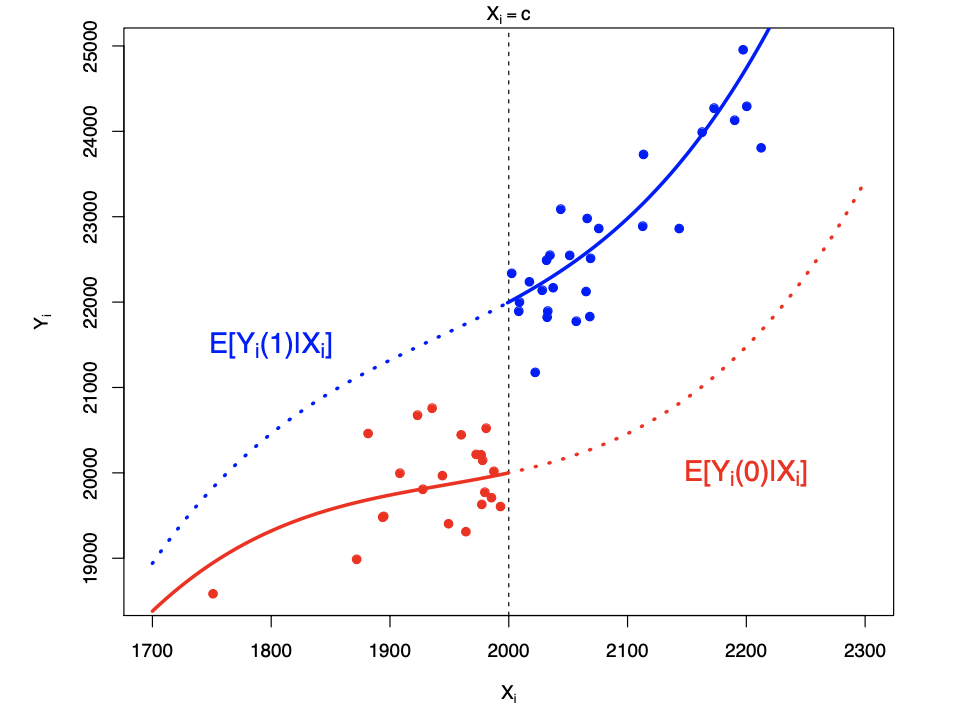
\includegraphics[height=.8\textheight]{figures/R2-2.png}
\end{center}
\end{frame}
%----------------------------------------------------------------
\subsection{Estimation}
\begin{frame}
\frametitle{Estimation of the ATE at the Threshold}
\vfill
\begin{enumerate} \vfill
\item Trim sample to window around threshold $c$ \vfill
\begin{itemize} \vfill
\item $c - \underline{h} \leq X_i \leq c + \overline{h}$ \vfill
\item Different methods for choosing width of window, $h$: \vfill
\item[] $\star$ Imbens-Kalyanaraman algorithm \citep{imbenskalyanaraman2012} \vfill
\item[] $\star$ Calonico, Cattaneo, and Titiunik algorithm  \citep{calonicoetal2014} \vfill
\end{itemize} \vfill
\item Recode running variable to $\widetilde{X_i} = X_i - c$ \vfill
\begin{itemize} \vfill
\item $\widetilde{X_i} = 0$ if $X_i=c$ \vfill
\item $\widetilde{X_i} > 0$ if $X_i>c$ and thus $Z_i=1$ \vfill
\item $\widetilde{X_i} < 0$ if $X_i<c$ and thus $Z_i=0$ \vfill
\end{itemize} \vfill
\item Choose model for $\E(Y_i \mid \tilde X_i)$: \vfill
\begin{itemize} \vfill
\item linear, common slope for $\E(Y_i \mid \widetilde{X}_i< 0)$ and $\E(Y_i \mid \widetilde{X}_i > 0)$ \vfill
\item Linear, different slopes \vfill
\item Local linear with kernel weights \vfill
\item[] \mh{Each model makes particular modeling assumptions} \vfill
\end{itemize} \vfill
\end{enumerate} \vfill
\end{frame}
%----------------------------------------------------------------
\begin{frame}
\frametitle{Estimation of the ATE at the Threshold: Choice of Kernel Weights}
\begin{center}
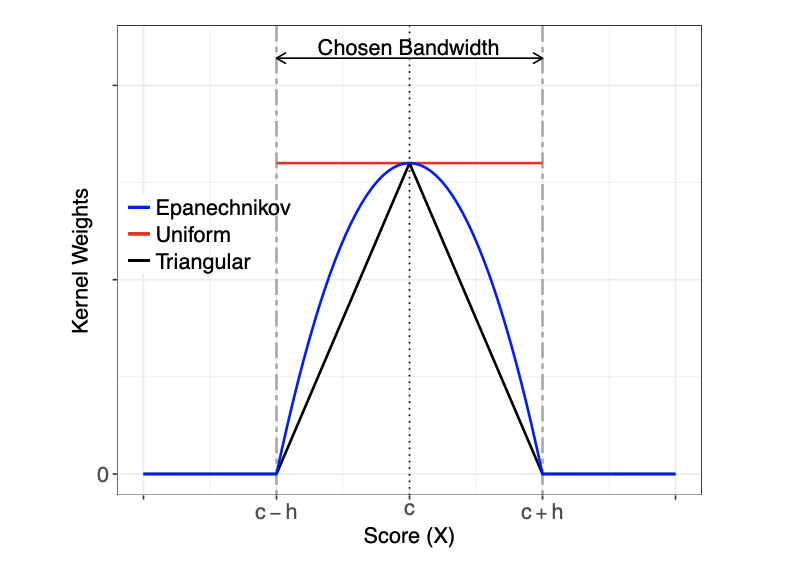
\includegraphics[height=3in, keepaspectratio=1]{figures/kernel.png}
\end{center}
\end{frame}
%----------------------------------------------------------------
\begin{frame}
\frametitle{Inference of the ATE at the Threshold}
\vfill
\begin{itemize} \vfill
\item Estimation typically uses model to predict potential outcomes at cutoff \vfill
\item Models (e.g., local linear regression) viewed as approximations \vfill
\item So construct confidence intervals robust to bias \citep[see][]{calonicoetal2014} \vfill
\item Use \texttt{R} packages \textrm{rdrobust} and \textrm{nprobust} + read \citet{calonicoetal2019} \vfill
\end{itemize} \vfill
\end{frame}
%----------------------------------------------------------------
\begin{frame}[allowframebreaks]
\frametitle{References} 
\scriptsize
\bibliographystyle{chicago}
\bibliography{rdd_bibliography}   % name your BibTeX data base
\end{frame}
%---------------------------------------------------------------
\end{document}